\begin{figure*}[tbp]
     \centering
     \begin{subfigure}[b]{0.33\textwidth}
        \centering
        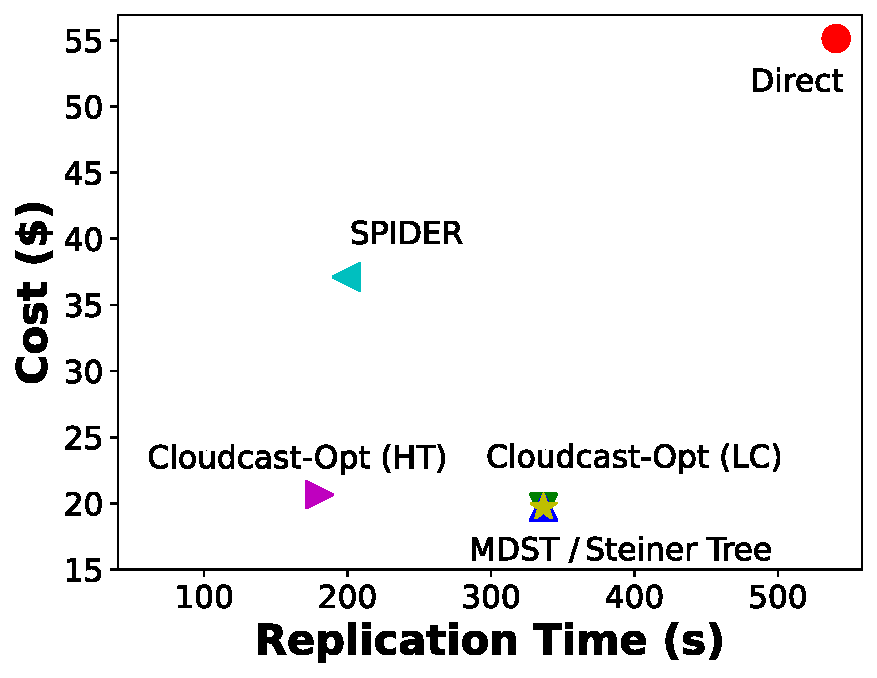
\includegraphics[width=\textwidth]{figures/aws.pdf}
        \caption{AWS Intra-Cloud}
        \label{fig:aws-intra-cloud}
    \end{subfigure}
    \hfill
    \begin{subfigure}[b]{0.33\textwidth}
        \centering
        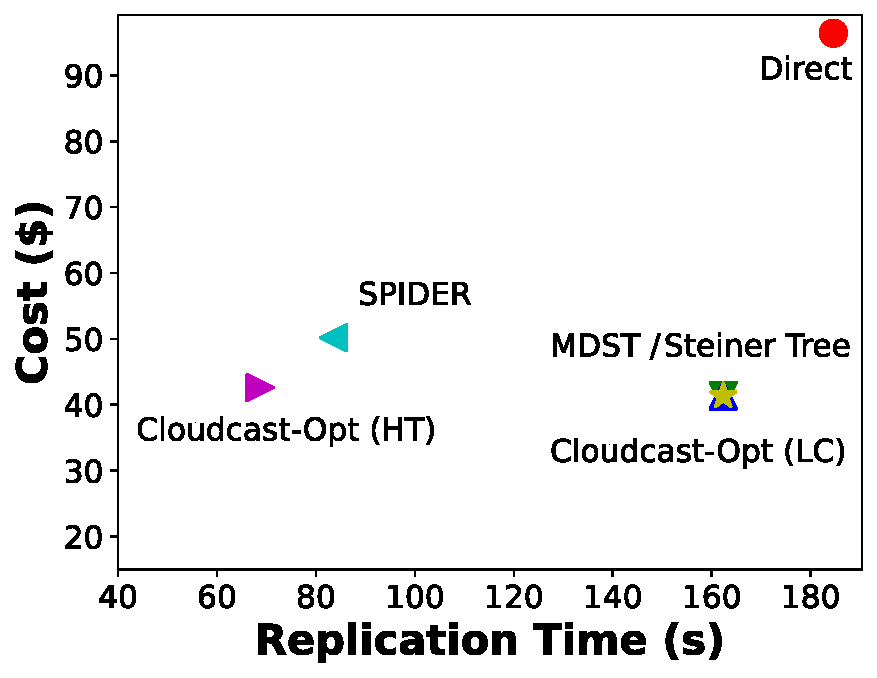
\includegraphics[width=\textwidth]{figures/azure.pdf}
        \caption{Azure Intra-Cloud}
        \label{fig:azure-intra-cloud}
    \end{subfigure}
    \hfill
    \begin{subfigure}[b]{0.33\textwidth}
        \centering
        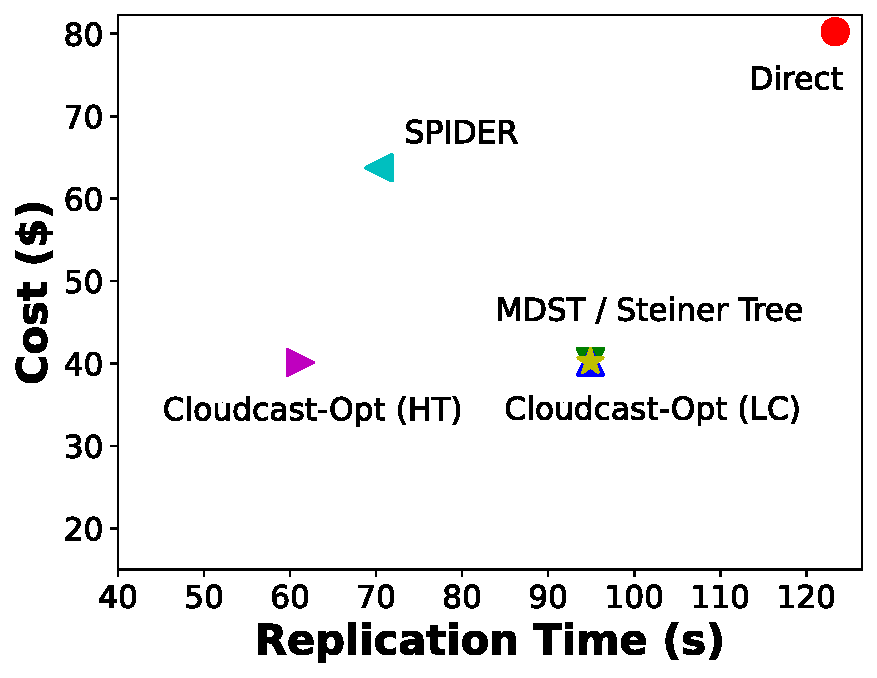
\includegraphics[width=\textwidth]{figures/gcp.pdf}
        \caption{GCP Intra-Cloud}
        \label{fig:gcp-intra-cloud}
    \end{subfigure}
    \hfill
    %\vspace{-2em}
    \caption{Intra-cloud multicast results for algorithms implemented on \sys{}.  
    %In all cases \sys{}-Opt is able to find significantly faster low-cost solutions where compared with existing techniques.  Furthermore, the MDST/Steiner Tree solution using ephemeral waypoints is able to consistently find the cost-optimal solution.  
    % \shu{we need to explain why we use these topologies, as well as why there are some variances in the running outcomes (e.g. SPIDER is closer to Cloudcast in Azure, or AWS runtime is much worse than the other cloud)}
    }
    \label{fig:intra-cloud}
\end{figure*}